This section presents the results of the proposed method applied to various datasets. The initial part of this section compares the proposed method with a related method for change point detection based on subspace identification using online SVD.~Artificial step detection highlights the significant differences in identifying subspaces using the two decomposition methods. Two real-world datasets are used to compare the performance of our proposed method with that of the alternative subspace identification method.

Secondly, we address the most challenging real-world dataset involving faulty HVAC operation detection in an industrial-scale battery energy storage system (BESS). The final subsection compares the proposed method with other methods used for change-point detection on benchmarking data of a simulated complex dynamical system with control (CATS) and a laboratory water circulation system (SKAB).

\subsection{Artificial steps detection}
Change-point detection can be simplified to finding temporal dynamics of a system not captured in data or acknowledged by the supervisory control system. A simple artificial dataset with steps and Gaussian noise can validate the proper functioning of the proposed method. This dataset, initially proposed in~\citet{Kawahara2007}, highlights our proposed variation of online DMD as superior to online singular value decomposition.

The dataset consists of 10,000 snapshots with nine steps of increasing size and distance from the original operation point after every 1,000 snapshots. Gaussian noise is added to target one of the weaknesses of subspace-identification-based methods.

The proposed method is compared to the one proposed by \citet{Kawahara2007} using the same hyperparameters, as listed in Table~\ref{table:kawahara_comp_hyperparameters}.

\begin{table}[ht]
    \caption{Hyperparameters used for comparison with online SVD based CPD.}\label{table:kawahara_comp_hyperparameters}
    \centering
    \begin{tabular}{l S[table-format=3.0]}
        \toprule
        \textbf{Hyperparameter} & \textbf{Value} \\
        \midrule
        \(r\)                   & 2              \\
        \(a\)                   & 100            \\
        \(b\)                   & 0              \\
        \(c\)                   & 100            \\
        \(d\)                   & 300            \\
        \(h\)                   & 80             \\
        \bottomrule
    \end{tabular}
\end{table}

The results, presented in Figure~\ref{fig:artificial_steps_detection}, show that while no method identified the first change-point at snapshot 1000, DMD-CPD discriminates minor change-points around the first operation point, with decreasing change-point statistics for subsequent detections. This decrease can be explained by the significant increase in absolute error between the original and reconstructed data, compared to the relative error between base and test sets, which decreases the residual of their division. Computing the difference of test and base set reconstruction errors, gives evidence to previous explanation. This relation of energy of the change-point detection to the actual dissimilarity of the data is a significant advantage of the proposed method over the deep learning techniques~\citep{DeRyck2021}. To sum up, the absolute dissimilarity of the data is reflected in the difference of the errors, while the relative dissimilarity is reflected in the error ratio.

The proposed method has a similar shape of statistics for error differencing to the error ratio statistics as the method proposed in \citet{Kawahara2007}, but with significantly better recognition of minor change points around the center of the dataset.

In both cases, the peak of the change-point statistics is delayed by \(c\) snapshots, which is expected due to the nature of CPD-DMD.~The exact delay allows for precisely pinpointing the change-point time from the data.

\begin{figure}[H]
    \centering
    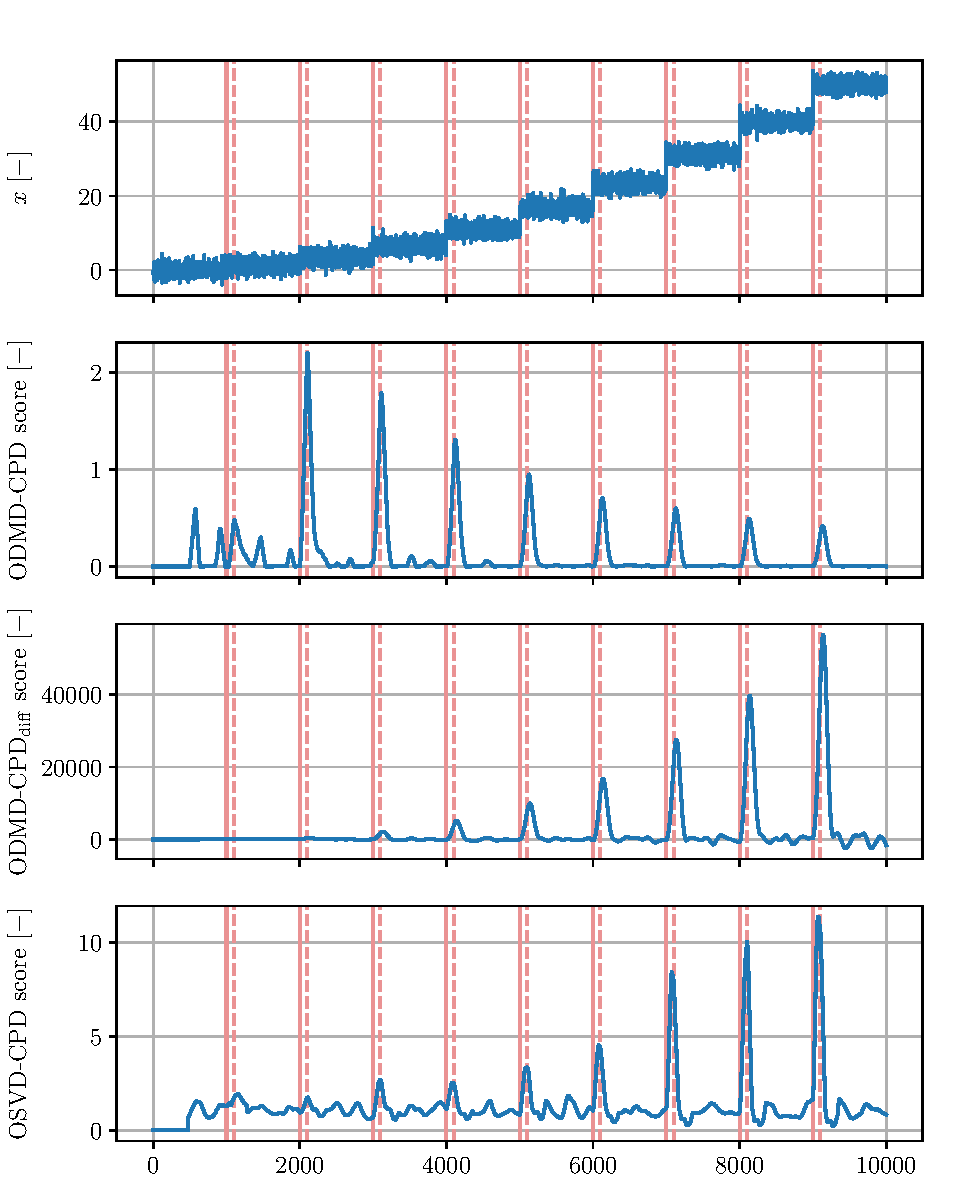
\includegraphics[width=\linewidth]{figures/y0-chd_r2_100_100-roll_301-dmd_w1.0-h80.pdf}
    \caption{Artificial steps detection.}\label{fig:artificial_steps_detection}
\end{figure}

\subsection{Sleep Stage Detection via Respiration Signal}
Identifying change points in real-world data is challenging due to cyclic, seasonal, and environmental effects. In this context, we use a dataset of respiration signals from a sleep stage detection task. The datasets represent respiration (thorax extension), sampled at 10 Hz from different subjects. The data are manually labeled by Dr.~J. Rittweger from the Institute for Physiology at the Free University of Berlin. For details, refer to the original publication~\citep{Keogh2005}. For comparison with online SVD, we use the same hyperparameters as in the previous section, listed in Table~\ref{table:kawahara_comp_hyperparameters}.

\paragraph{NPRS43}
The comparison results of experiments conducted on NPRS43 dataset are presented in Figure~\ref{fig:nprs43}. This dataset spans approximately 7 minutes of sleep respiration signals of a subject. The subject is in stage II deep sleep for the first 5 minutes, then transitions through a short awake stage of approximately 1 minute to the stage I sleep. The transitions are marked as red vertical lines in the plot. Due to the size of the test set, the peak of change-point statistics is delayed by \(c\) snapshots and marked as red dashed vertical lines.

Both methods identify the first transition from stage II to the awake state with a peak of statistics delayed by \(c\). While SVD fails in recognizing the second transition, our method displays increased score with significant delay after the transition. Since the delay is longer than \(a + c\), it could be regarded as a false positive detection of a change point. Nonetheless, by visually examining data after the ground truth label, it could be argued that second transition occurs in more gradual manner and spans multiple breathing cycles, two with very short thrax extensions after ground truth label, followed by two with lerger thrax extensions and ended by two very large extensions. Our method seems to capture middle point of this gradual transition as a reference and learning windows cross the first transition point. Validity of this reasoning was not supported by the

\begin{figure}
    \centering
    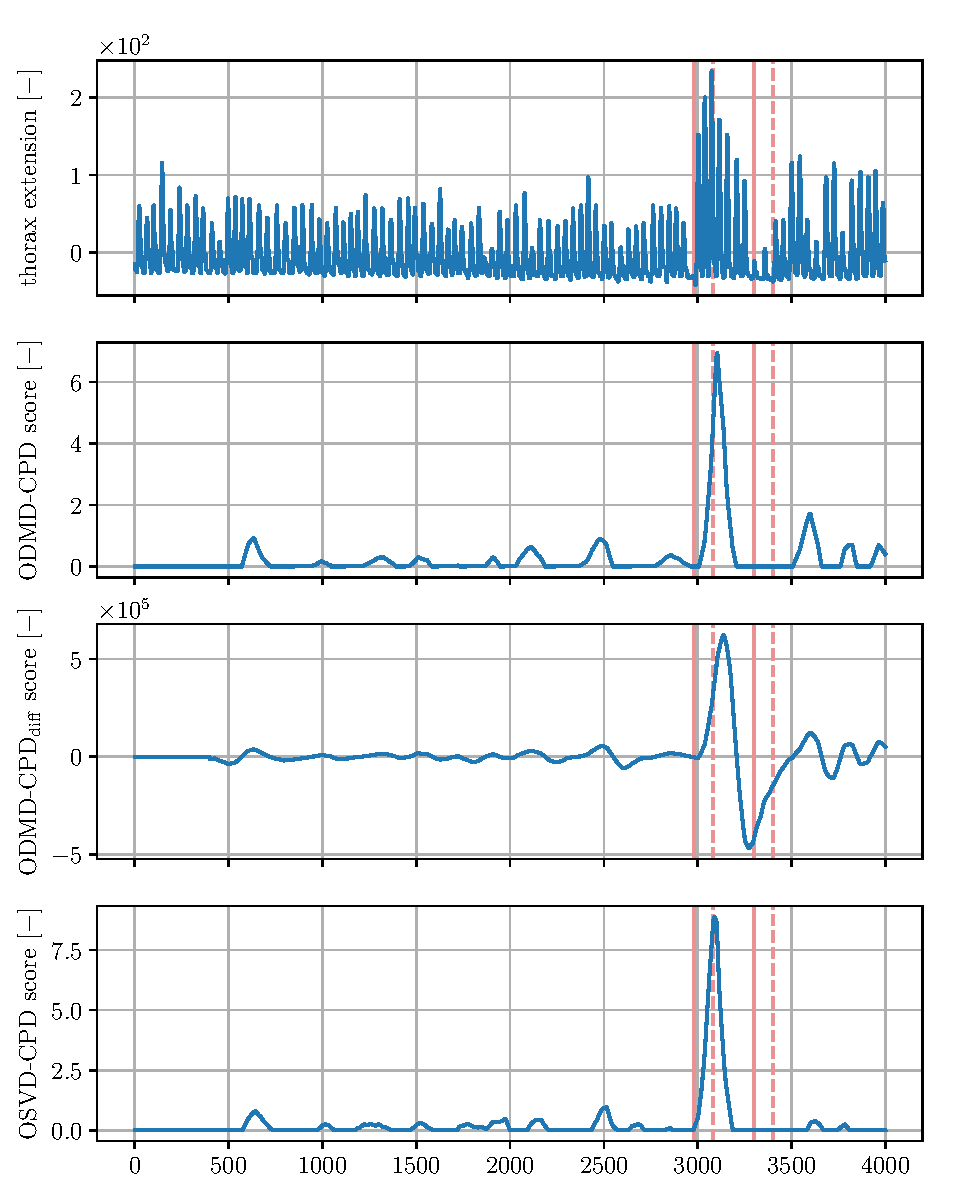
\includegraphics[width=\linewidth]{figures/nprs43-chd_r2-roll_301-dmd_w1.0-h80.pdf}
    \caption{NPRS43: Sleep stage transition detection based on respiration data (1). Change score is evaluated for: proposed method as presented in Section~\ref{sec:method} (2), proposed method evaluating score as the difference of errors (3), and reference method using online SVD (4).}\label{fig:nprs43}
\end{figure}

\paragraph{NPRS44}
The comparison results of experiments conducted on NPRS44 dataset are presented in Figure~\ref{fig:nprs44}. This dataset spans approximately 11 minutes of sleep respiration signals of a subject. The subject is in stage II deep sleep for the first 4 minutes, then transitions through the stage I sleep, indicated by shallow breathing, for approximately 4 minutes to an awake state. The transitions are marked as red vertical lines, and the ideal change statistics peak as grey lines in the plot.

Both methods identify the transitions present in the dataset with high discrimination capacity. CPD-DMD has significantly fewer sharp peaks in areas where a transition is not anticipated compared to the SVD-based method. Moreover, CPD-DMD captures the second transition with higher prominence and achieves peak detection with a delay of exactly \(c\) snapshots. Under the same parametrization, CPD-DMD shows smoother scores and slightly better discrimination of the transitions.

\begin{figure}[H]
    \centering
    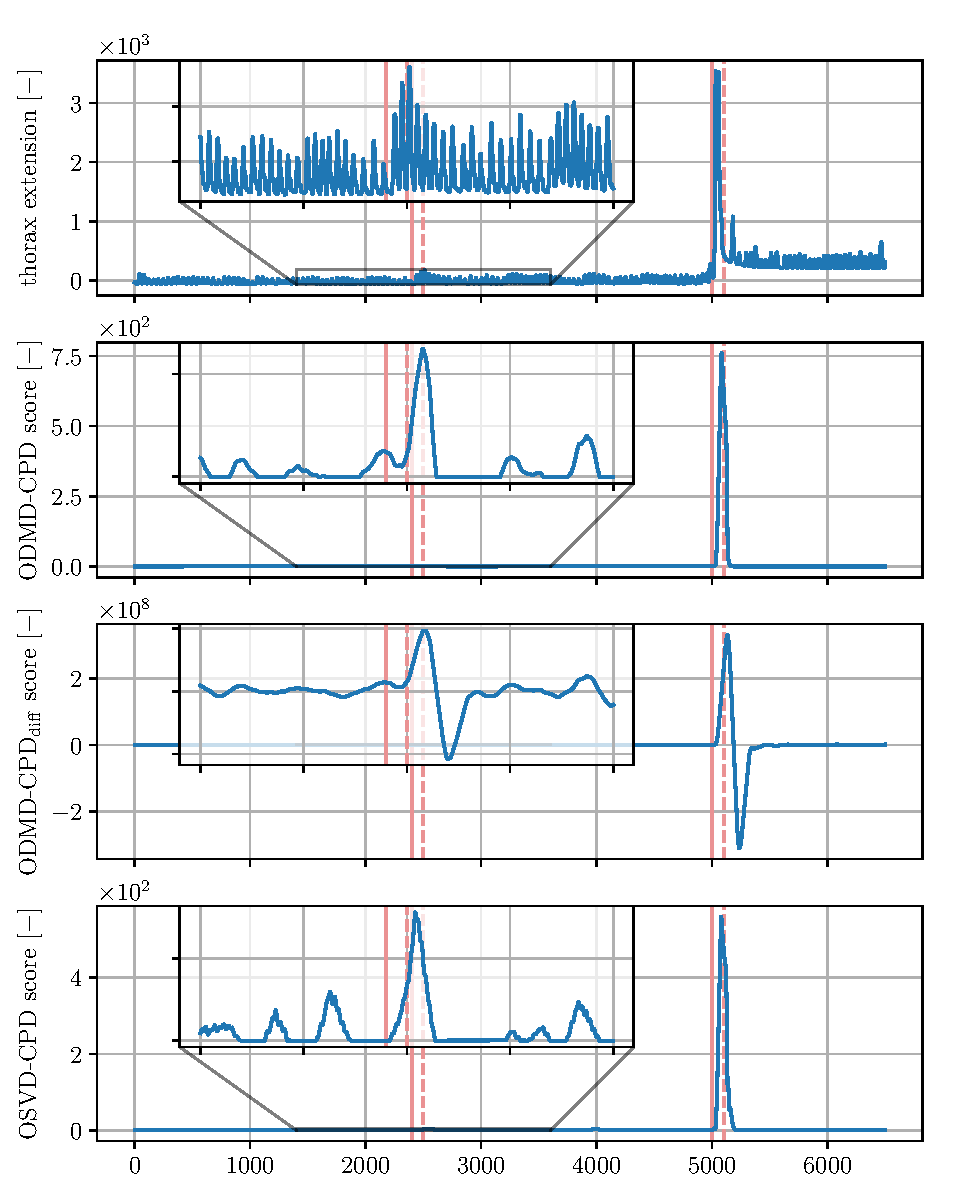
\includegraphics[width=\linewidth]{figures/nprs44-chd_r2-roll_301-dmd_w1.0-h80.pdf}
    \caption{NPRS434: Sleep stage transition detection based on respiration data (1). Change score is evaluated for: proposed method as presented in Section~\ref{sec:method} (2), proposed method evaluating score as the difference of errors (3), and reference method using online SVD (4).}\label{fig:nprs44}
\end{figure}

\subsection{BESS --- Faulty HVAC Operation Detection}
This case study demonstrates detection performance on a real-world dataset of faulty HVAC operation in an industrial-scale battery energy storage system (BESS). The studied BESS has an installed capacity of 151 kWh distributed among ten modules with 20 Li-ion NMC cells. A hardware fault occurred on one of the module's cooling fans on 23rd August 2023 at 17:12:30. To protect the profitability of the BESS for the end user, the faulty BESS was operated securely until the fault was fixed. This case study aims to detect the transition from normal to faulty operation of the HVAC system based on temperature profile monitoring. The dataset is provided by the BESS operator and normalized to protect sensitive business information. It captures snapshots of six spatially distributed temperature sensors of the targeted BESS module operation at approximately 30-second intervals.

The selection of hyperparameters demonstrates the intuitiveness of parameter selection. The BESS is utilized in an industrial setting for availability time-shifting of energy generated by a solar power plant, subject to daily seasonality and weekly periodicity. The learning window \(d\) is set for 24 hours to reflect these patterns and track weekday and weekend operations well. The maximum C-rate of the BESS is 1.0, defining another important hourly time constant. With this knowledge, we can minimize the impact of charging events on change-point detection statistics; \(a\) and \(c\) window sizes are set to double the fastest charging rate, 240 samples, corresponding to 2 hours of operation. The number of time delays in the embedded matrix reflects the known dynamics of the system; hence, \(h\) is set to 240 samples.

The results of the detection experiment on simulated data streaming from the BESS history replay, presented in Figure~\ref{fig:bess}, show that before the actual occurrence of the fault, the system detects multiple events of abnormal operation with a source other than the identified dynamical system from the data. The proposed method accurately detects the transition from normal to faulty operation of the HVAC system with high accuracy and low false positive rate, with the peak of change-point statistics delayed by \(c\) snapshots.

The proposed method detected three periods related to the transient normal behavior of the HVAC system, marked as change points. The alternative error evaluation method shows that we can detect both the transition from normal to faulty operation and vice versa. Due to the precise discrimination of faulty operation from normal, operators may regard initial peaks in change-point statistics as possible indicators of an approaching fault. This could be valuable for early detection and prevention of catastrophic consequences and maintenance planning. The positions of the potential fault precursors match the detected anomalies in~\citet{Wadinger2024}. This is particularly interesting from the perspective of cross-validating the methods and giving more credibility to regard these events as precursors of something more serious.

\begin{figure}[H]
    \centering
    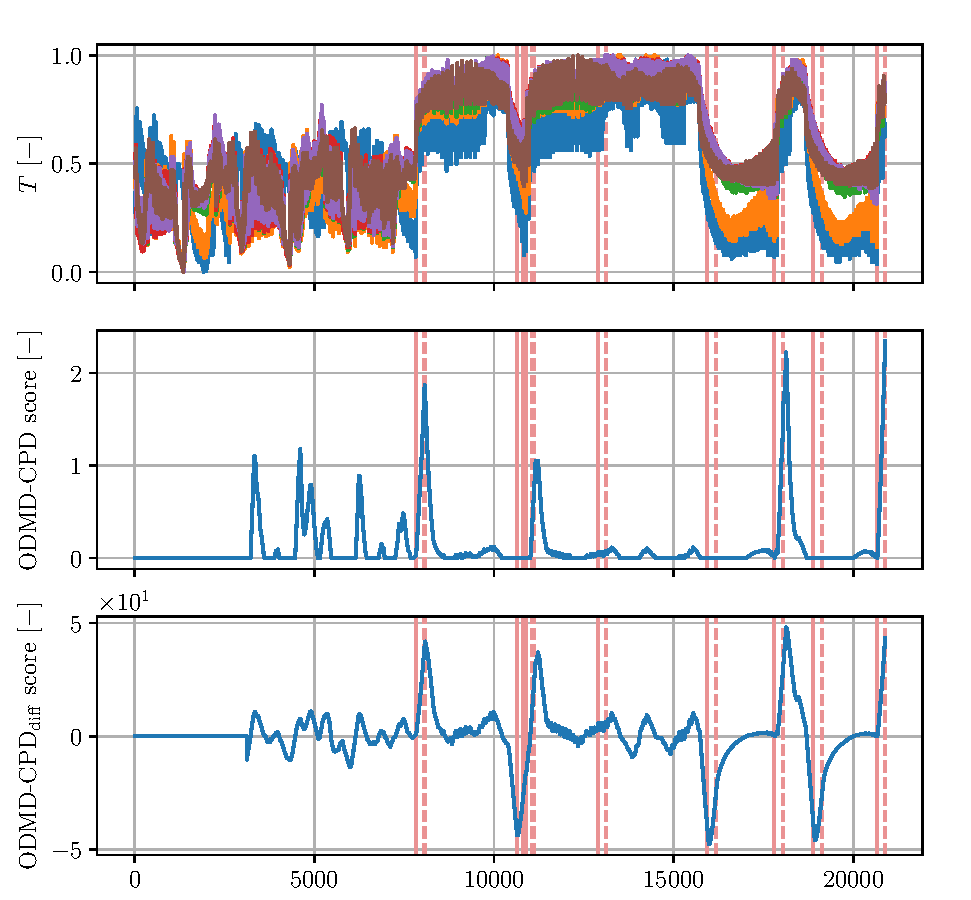
\includegraphics[width=\linewidth]{figures/bess-chd_p10-l2880_b240_t240roll_2880-dmd_w1.0-hx20.pdf}
    \caption{Faulty operation of HVAC in BESS results in increased operation temperature.}\label{fig:bess}
\end{figure}


\subsection{Laboratory Water Circulation System (SKAB)}
In this section, we compare the performance of the proposed method with commonly used change-point detection methods on a benchmark real-world dataset of a laboratory water circulation system (SKAB)~\citep{Katser2020}. The dataset represents a well-described industrial system with multiple sensors and well-defined operational and fault states characterized by collective anomalies or change points, as well as transitions between these states.

\citet{Katser2020} compare methodswith default hyperparameters, which are listed in Table~\ref{table:comparison-models}, using the first 400 snapshots of each dataset as a training part. We follow the same procedure, and for CPD-DMD hyperparameters with task-specific tuning requirements, we use the training set of samples as a history of snapshots to establish the parameters.

\begin{table}[H]
    \caption{List of reference method and sources}\label{table:comparison-models}
    \centering
    \begin{tabular}{l l S[table-format=3.0]}
        \toprule
        \textbf{Algorithm} & \textbf{Source}       \\
        \midrule
        Conv-AE            & \citet{Pavithra2020}  \\
        Isolation forest   & \citet{Liu2008}       \\
        LSTM-AE            & \citet{Chollet2016}   \\
        MSCRED             & \citet{ZhangCh2019}   \\
        MSET               & \citet{Gross2000}     \\
        T-squared          & \citet{Hotelling1947} \\
        T-squared+Q (PCA)  & \citet{JoeQin2003}    \\
        Vanilla AE         & \citet{Chen2017}      \\
        Vanilla LSTM       & \citet{Filonov2016}   \\
        \bottomrule
    \end{tabular}
\end{table}

The evaluation is performed using NAB metrics presented in the work of~\citet{Ahmad2017}. These metrics operate over a window of snapshots. This window is centered around the change point to establish metrics for reference methods. Nevertheless, from the definition of the change-point and the utilization of the window for scoring (please refer to the paper by~\citet{Lavin2015}), it is evident that the perfect detector should detect a change-point half of the window size snapshots before the change-points actual occurrence. Since the start of the transition towards the faulty state is marked as anomalous in the dataset, as seen in Figure~\ref{fig:scab_interpretation}, we stipulate that the detection before the start of the transition should be regarded as a false positive. Therefore, we modify the original evaluation metrics to observe the snapshots window after the change-point and evaluate the models' performance.

To ensure reproducibility and consistency, we created a fork of the original repository available at \url{https://github.com/MarekWadinger/SKAB}.

\begin{figure}[H]
    \centering
    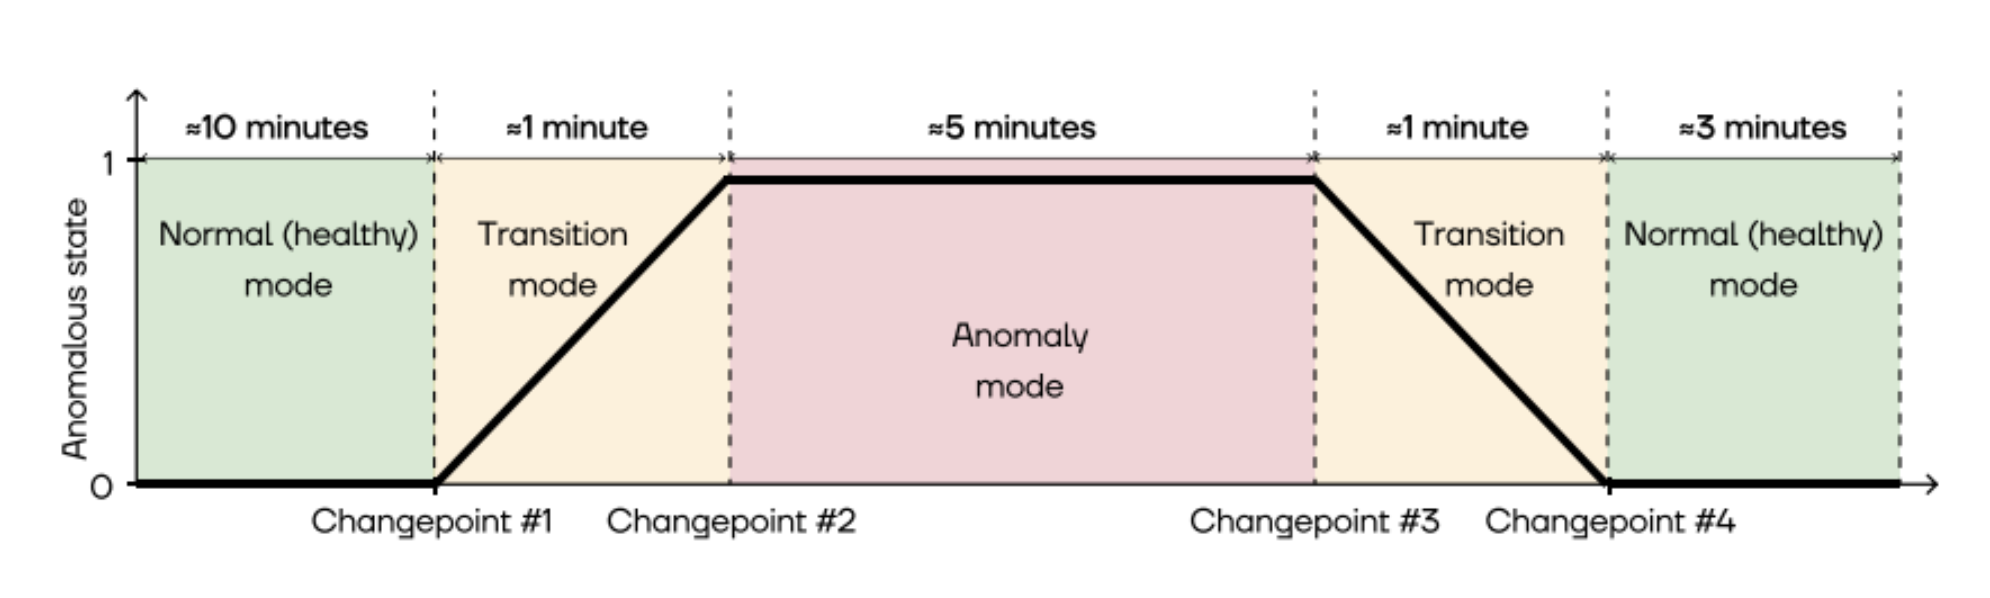
\includegraphics[width=\linewidth]{figures/scab-interpretation.png}
    \caption{Description of anomaly mode, transition, and positions of marked change points.}\label{fig:scab_interpretation}
\end{figure}

The results of experiments with modified evaluation, presented in Table~\ref{table:skab_cpd_comparison-own}, show that the proposed method outperforms the reference methods in terms of standard NAB score except MSCRED.~Nevertheless, it has a lower false positive rate than MSCRED, which is presented in terms of both score and the number of false positives. Conv-AE, LSTM-AE, and Isolation Forest all present a far lower number of false positives than the proposed method. The difference in the low FP metric is insignificant, indicating a longer duration of false alarms. Our proposed method and MSCRED have the lowest number of missed change points, making them more suitable methods for safety-critical systems where missed alarms may result in catastrophic consequences. Perhaps most interesting is the score of the perfect detector, which is not 100 as expected. This indicates that the standard NAB score does not guarantee a 100 for the perfect detector, which is essential to consider when evaluating the relative performance of the methods with respect to the perfect detector.

\begin{table}[H]
    \caption{Comparison of different algorithms based on NAB metrics. Two highest scores are highlighted}\label{table:skab_cpd_comparison-own}
    \centering
    \begin{tabular}{l *3{S[table-format=3.2]} *2{S[table-format=3.0]}}
        \toprule
        \textbf{Algorithm}           &
        \multicolumn{1}{p{1.7cm}}{\centering \textbf{NAB}                                                           \\ (standard)} &
        \multicolumn{1}{p{1.7cm}}{\centering \textbf{NAB}                                                           \\ (low FP)} &
        \multicolumn{1}{p{1.7cm}}{\centering \textbf{NAB}                                                           \\ (low FN)} &
        \textbf{FNs}                 &
        \textbf{FPs}
        \\
        \midrule
        Perfect detector             & 54.77          & 54.11          & 56.99          & 49          & 0           \\
        \midrule
        MSCRED                       & \textbf{32.42} & 16.53          & \textbf{40.28} & \textbf{55} & 342         \\
        \textbf{CPD-DMD (alt.)}      & \textbf{30.29} & 18.31          & \textbf{37.78} & \textbf{60} & 250         \\
        \textbf{CPD-DMD (t=0)}       & 29.68          & 17.48          & 37.37          & \textbf{60} & 254         \\
        \textbf{CPD-DMD (alt., t=0)} & 29.68          & 17.48          & 37.37          & \textbf{60} & 254         \\
        \textbf{CPD-DMD}             & 39.84          & 23.66          & 50.18          & 37          & 336         \\  % ref 120, test 60
        Isolation forest             & 26.16          & 19.50          & 30.82          & 76          & 135         \\
        T-squared+Q (PCA)            & 25.35          & 14.51          & 31.33          & 72          & 232         \\
        Conv-AE                      & 23.61          & \textbf{21.54} & 27.55          & 82          & \textbf{23} \\
        LSTM-AE                      & 23.51          & \textbf{20.11} & 25.91          & 88          & 69          \\
        T-squared                    & 19.54          & 10.20          & 24.31          & 70          & 106         \\
        MSET                         & 13.84          & 10.22          & 17.37          & 96          & \textbf{66} \\
        Vanilla AE                   & 11.41          & 6.53           & 13.91          & 103         & 106         \\
        Vanilla LSTM                 & 11.31          & -3.80          & 17.25          & 90          & 342         \\
        \midrule
        % Always positive              & 0              & 0              & 0              & 0           & 1           \\
        Null detector                & 0              & 0              & 0              & 127         & 0           \\
        \bottomrule
    \end{tabular}
\end{table}


\subsection{Simulated Complex Dynamical System with Control (CATS)}
This section evaluates the Controlled Anomalies Time Series (CATS) Dataset in \citet{Schmidl2022}. The dataset shows a simulation of a complex dynamical system with 200 injected anomalies, consisting of commands, external stimuli, and 5 milion snapshots of telemetry sampled at 1 Hz. While the generating mechanism is not described, the availability of the benchmark dataset, including the control action signals, makes it a good candidate for evaluating the proposed method. The dataset is meant for anomaly detection algorithms but contains numerous sequences of anomalous behavior. Compared to SKAB, this dataset has a far lower contamination level of 3.8\%, making it more suitable for evaluating the change-point detection performance, where events of change are underrepresented.

The evaluation uses the same metrics as the previous case study on a resampled dataset to 1-minute intervals, with a median taken for both features and targets. No public background on the generating mechanism complicated the hyperparameter selection. Based on the 58-day timespan captured in the dataset, we selected one day as the learning window and set the number of time delays to 4 hours, with a maximum limit of the final number of features set to 60. The reference window is double the size of the test window, 10 hours for the former and 5 hours for the latter. The ranks of the DMD were set to 10 and 4 for the states and control inputs, respectively.

The results of experiments, presented in Table~\ref{table:cats_cpd_comparison}, show that the proposed method outperforms all reference methods but MSCRED in terms of the standard NAB score evaluated on a 5-hour window starting to the right of the actual anomaly. It is worth stating that while our proposed method and other reference methods completed the experiment within 1 hour, it took almost 24 hours for MSCRED. This means that it requires roughly one second per snapshot to process the data, which would challenge MSCRED's applicability in hard real-time scenarios with the original frequency of 1 Hz. Two best methods in terms of the standard NAB score also display highest number of false positives, which is a trade-off between the number of missed change points and false alarms. Other methods with lower false positive rates have higher number of missed change points.

In the given settings, our proposed method balances well between false positives and false negatives, with the lowest number of missed change points. The results indicate that the proposed method is capable of detecting change points in the complex dynamical system and can employ information about control inputs.

\begin{table}[H]
    \caption{Comparison of different algorithms based on NAB metrics.}\label{table:cats_cpd_comparison}
    \centering
    \begin{tabular}{l *3{S[table-format=3.2]} *2{S[table-format=3.0]}}
        \toprule
        \textbf{Algorithm}           &
        \multicolumn{1}{p{1.7cm}}{\centering \textbf{NAB}                                                           \\ (standard)} &
        \multicolumn{1}{p{1.7cm}}{\centering \textbf{NAB}                                                           \\ (low FP)} &
        \multicolumn{1}{p{1.7cm}}{\centering \textbf{NAB}                                                           \\ (low FN)} &
        \textbf{FNs}                 &
        \textbf{FPs}
        \\
        \midrule
        Perfect detector             & 30.21          & 29.89          & 31.28          & 265          & 0          \\
        \midrule
        MSCRED                       & \textbf{37.19} & 13.46          & \textbf{47.18} & \textbf{130} & 1659       \\
        \textbf{CPD-DMD (alt.)}      & \textbf{22.51} & 18.13          & \textbf{25.65} & \textbf{271} & 277        \\
        \textbf{CPD-DMD (t=0)}       & 22.46          & \textbf{18.15} & 25.61          & \textbf{271} & 271        \\
        \textbf{CPD-DMD (alt., t=0)} & 22.46          & \textbf{18.15} & 25.61          & \textbf{271} & 271        \\
        \textbf{CPD-DMD}             & 13.40          & 11.69          & 15.05          & 325          & 98         \\
        Isolation forest (c=3.8\%)   & 17.81          & 15.84          & 20.00          & 301          & 106        \\
        T-squared+Q (PCA)            & 11.80          & 11.40          & 12.30          & 345          & 20         \\
        Conv-AE                      & 0.15           & 0.14           & 0.18           & 397          & \textbf{0} \\
        LSTM-AE                      & 11.39          & 11.26          & 11.69          & 349          & \textbf{3} \\
        T-squared                    & 15.15          & 14.98          & 15.71          & 331          & \textbf{0} \\
        MSET                         & 14.48          & 13.43          & 15.60          & 327          & 58         \\
        Vanilla AE                   & 2.52           & 2.44           & 2.77           & 385          & \textbf{0} \\
        Vanilla LSTM                 & 0.73           & 0.70           & 0.82           & 394          & \textbf{0} \\
        \midrule
        % Always positive              & 0              & 0              & 0              & 0            & 1          \\
        Null detector                & 0              & 0              & 0              & 398          & 0          \\
        \bottomrule
    \end{tabular}
\end{table}
